\documentclass[15pt]{article}
\usepackage[utf8]{inputenc}

\usepackage[total={18.5cm,22.5cm}]{geometry}
\usepackage[spanish]{babel}
\usepackage{geometry} 
\usepackage[dvipsnames]{xcolor}
\usepackage{graphicx} %imágenes
\usepackage{caption}
\usepackage{hyperref}
\usepackage{fancyhdr}%encabezados
\pagestyle{fancy}
\hypersetup{
    colorlinks=true,
    urlcolor=blue,
    }

\urlstyle{same}

\title{\textbf{Analizador de textos con Python}}
\author{Méndez González Romina Estephania\\
Rodríguez Castillo Jordan Ricardo\\
Moreno Aguilar Diego Denilson}
\date{Diciembre de 2022}

\begin{document}

\maketitle

\section*{\Large{Resumen}}

En este proyecto hemos optado por la elaboración de una herramienta útil y fácil de programar, sin muchos enredos, tal como pretende ser el mismo lenguaje Pyhton. Con el empleo de comandos sencillos hemos podido darresolución a una tarea, el conteo de caracteres y palabras, que para el humano sería tardada y tediosa, en especial para grandes volumenes de texto.

\section*{\Large{Introducción}}

\subsection*{Sobre los analizadores de texto}

Un analizador de textos es un programa que interactúa con un texto para brindarnos información de interés sobre el mismo. Esto lo hace, obviamente, de forma cuantitativa, dándonos datos como:

\begin{itemize}

    \item Frecuencia de frases, cuántas veces se repite una frase en cierto intervalo del texto. Cómo no, también podemos hacer lo mismo con palabras individuales y, claro, también con caracteres individuales.
    \item Número de caracteres totales en cierto intervalo, el intervalo puede ser todo el texto.
    \item Longitud promedio de las palabras en el texto.
    \item Palabra más larga, más corta o más usada.
    
\end{itemize}

En este caso sólo nos interesa el saber cuántas de cada letra a seleccionar se hallan en nuestro texto, la cantidad de palabras que hay en el mismo y la primera y última letra del mismo.

\subsection*{Objetivo/Motivación}

Como ya se habrá podido intuir previamente, el darle una tarea a un programa que para nosotros sería tardada e incluso sujeta a errores, tiene gran importancia y muchas implicaciones. A este punto nos es obvio que estaimportancia radica en la rapidez, eficiencia y capacidad para manejar volúmenes grandes de información de los programas de computadora (en especial sobre las de los humanos.\\

Yendo un poco más allá de lo obvio y en defensa de las capacidades humanas, podemos decir que algo que sí podemos hacer es combinar estos pequeños y sencillos comandos en otras tareas y otros contextos, totalmente distintos al de analizar las palabras en un texto, para crear herramientas aún más útiles y complejas. \\

Entender la sintaxis de los comandos aquí empleados nos permitirá usarlos posteriormente junto a otros más para poder resolver tareas cada vez más complejas y tardadas. Cada vez hacer las cosas más eficientemente y, supuestamente, de mejor forma.\\

\hspace{-15pt}\textcolor{Blue}{\rule{18.5cm}{1pt}}
\vspace{3pt}

\textcolor{Blue}{Antes mencionábamos que existen implicaciones de la acción de darle una tarea que previamente era realizada por humanos a un programa o una máquina. Mientras que estas acciones pueden parecerles totalmente positivas a algunos, cabe decir que siempre es posible preguntarse por si esto es 100\% positivo.} \\

\textcolor{Blue}{El facilitamiento de las tareas no está determinado, pues, puede ser nuestra salida de la obscuridad, como nuestra perdición. La mejor ejemplo de una salida de la obscuridad por medio de la tecnología es precisamente esto, el lenguaje y la escritura. El mejor ejemplo de la perdición por medio de entregar nuestras acciones a una interpretación ingenua de la tecnología es la pérdida de trabajos o quizá la pérdida de la privacidad precisamente por programas de análisis de datos. Las ventajas de la automatización pueden parecer grandes en teoría, pero en el mundo real no se ha progresado a jornadas laborales cortas, abundancia alimenticia, transición hacia el interés por el arte o las humanidades (hoy es precisamente cuando menos eso es el caso), bajos costos de producción o menos estrés al trabajar. Parece ser que incluso hoy se vive cada vez más tiempo en el trabajo, con menos abundancia, con más estrés y con mayor ansiedad, tal vez debido a la rapidez que induce la tecnología sobre nosotros.}\\

\hspace{-15pt}\textcolor{Blue}{\rule{18.5cm}{1pt}}

\vspace{15pt}
\section*{\Large{Cuerpo/Programa}}

\begin{figure}[h]
\centering
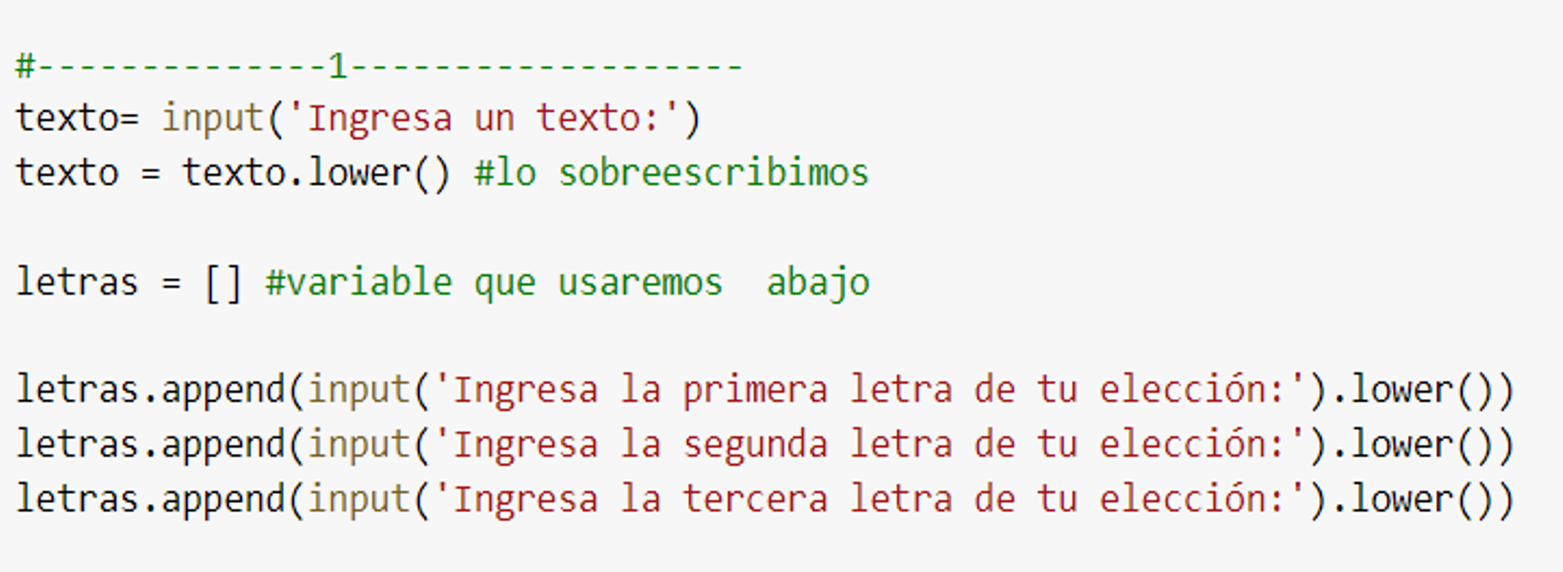
\includegraphics[scale=0.35]{Parte1.png}
\end{figure}

\begin{itemize}

    \item La estructura imput() permite al usuario introducir información y guardarla para después.
    \item La estructura .lower() transforma el texto a minúsculas, en este caso es aplicado a ``texto".
    \item La estructura .append() modifica una lista al añadir lo que esté dentro del paréntesis a la lista.
    \item Después, con la acción letras = [] definimos \textbf{letras} como una lista, por ahora, vacía.
    \item Con los siguientes 3 comandos de tipo:\\
    
    letras.append(input('Ingresa la primera letra de tu elección:').lower())\\
    
    Lo que hacemos es modificar la lista \textbf{letras} para que se añada el valor que ingrese el usuario.

\end{itemize}

\newpage

\begin{figure}[h]
\centering
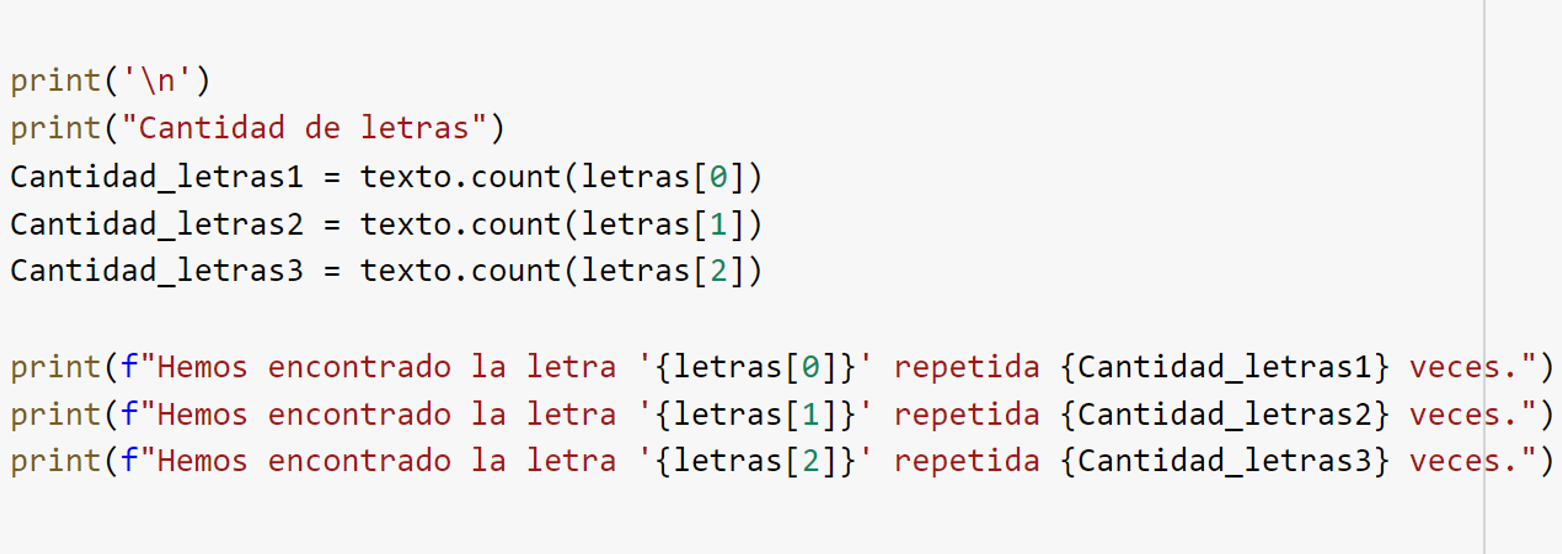
\includegraphics[scale=0.35]{Parte2.png}
\end{figure}

\begin{itemize}

    \item Con n creamos un salto de línea.
    \item Con los siguientes 3 comandos tipo:\\
    
    CantidadLetras1 = texto.count(letras[0])\\
    
    Lo que hacemos es definir la variable \textbf{CantidadLetras1} como el número de veces que aparece el elemento 0 de la lista \textbf{letras} dentro de ``texto".\\

    Esto se hace al ejecutar el comando .count(), que cuenta cuántos elementos iguales a lo que está dentro del paréntesis (en este caso, el elemento 0 de la lista \textbf{letras}, o sea, la primera letra que elegimos), sobre el elemento ``texto".
    \item Con los siguientes 3 comandos tipo:\\
    
    print(f"Hemos encontrado la letra '{letras[0]}' repetida {CantidadLetras1} veces.")\\

    Lo que hacemos es imprimir que se ha encontrado la entrada 0 de la lista \textbf{letras}, o sea, la primer letra que el usuario introdujo, repetida \textbf{CantidadLetras1} (variable que definimos anteriormente) veces dentro de ``texto".

\end{itemize}

\begin{figure}[h]
\centering
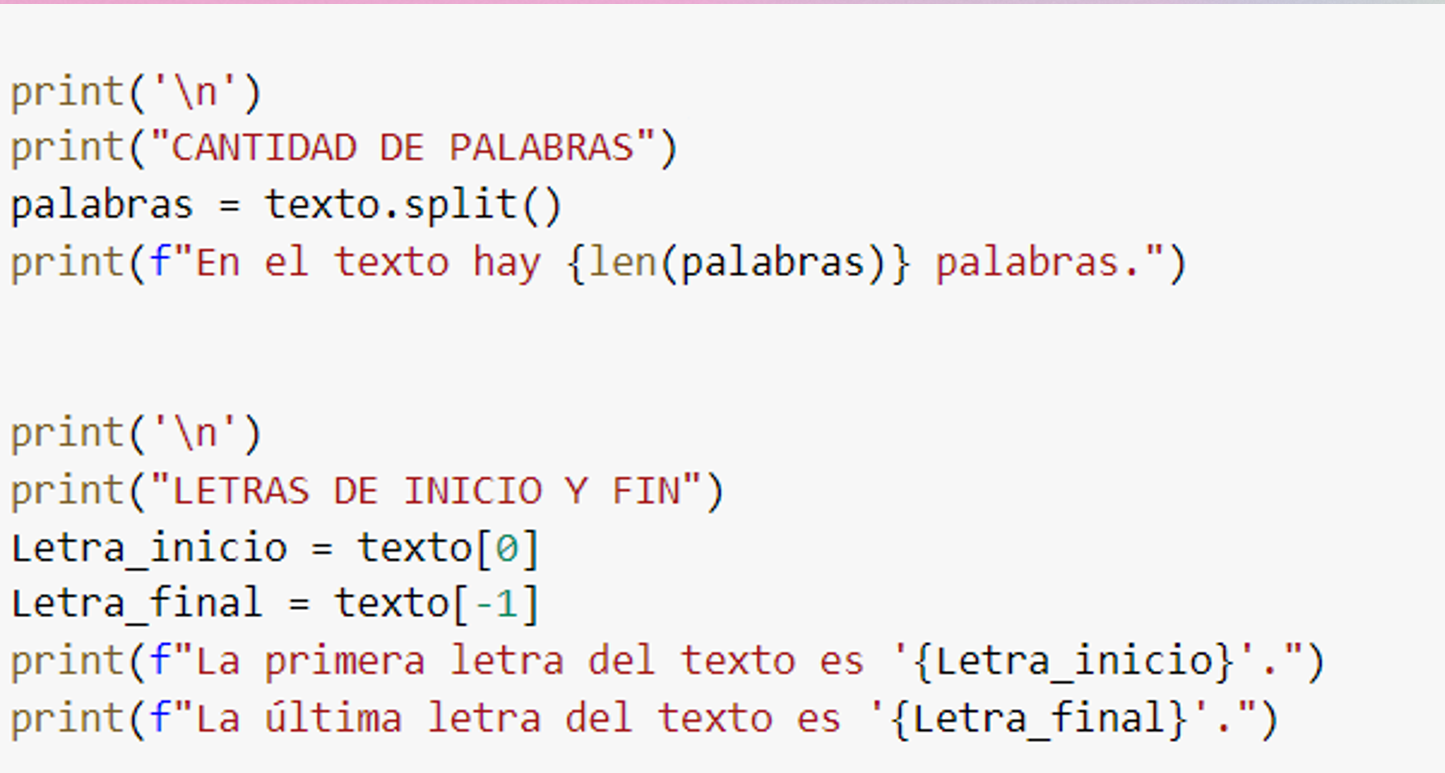
\includegraphics[scale=0.35]{Parte3.png}
\end{figure}

\begin{itemize}

    \item De la misma forma que antes, el print acompañado del n genera un salto de línea
    \item El siguiente comando importante es:

    \textbf{palabras = texto.split()}


    ``palabra'' es el nombre de la variable por definir que estará afectando al texto, cambiando así, al texto en una lista separando las palabras que tomará como elementos.

    \item Las últimas variables cumplen la misma función y trabajan bajo la misma instrucción.\newline

    en el caso de \textbf{Letra\_inicio = texto [ 0 ] } muestra la primera letra del texto \newline

    Y en el caso de \textbf{Letra\_final = texto [-1]} devuelve la última letra del texto

    \item Los ``print'' restantes agregan al código la explicación de lo que significa cada dato y dándole un formato general para que solamente se llene con la informació que corresponda para cada texto que se analice.

\end{itemize}

\section*{\Large{Resultados}}

\begin{figure}[h]
\centering
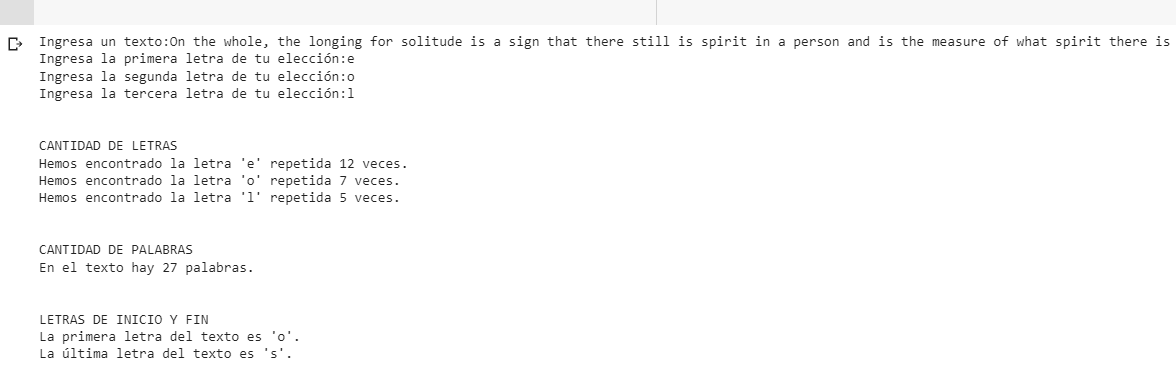
\includegraphics[scale=0.53]{Result.png}
\end{figure}

Al introducir una maravillosa cita ``On the whole, the longing for solitude is a sign that there still is spirit in a person and is the measure of what spirit there is" (En general, el anhelo por la soledad es signo de que aún hay espíritu en una persona y es la medidad de qué espíritu hay), obtenemos: \\

\noindent Letra \textbf{e}: 12 veces \\
Letra \textbf{o}: 7 veces \\
Letra \textbf{l}: 5 veces \\

\noindent Cantidad de palabras: \textbf{27} \\

\noindent Letra inicial: \textbf{o} \\
Letra final: \textbf{s} \\

\section*{\Large{Conclusiones}}

El programa funciona tanto para textos cortos como para citas enteras, acortando efectivamente el tiempo que tardamos en realizar la acción y reduciendo las probabilidades de que fallemos a 0 (si es que el código está bien escrito). El analizador de textos aquí presentado puede ser útil a la hora de contar las palabras en un ensayo o tesis (tarea que no es infrecuente) de manera sumamente fácil, también al contar las veces que se repite una secuencia de letras dentro del texto.\\
Igualmente sirve para ejemplificar cómo comandos individuales pueden configurarse de tal forma que nos sean útiles. En general, las herramientas que nos acorten el tiempo al realizar una tarea o la hagan menos propensa a errores, se puede decir que son ``benéficas". \\

\hspace{-15pt}\textcolor{Blue}{\rule{18.5cm}{1pt}}
\vspace{3pt}

\textcolor{Blue}{Aún más en general, quizá cabe decir que la elaboración de herramientas que ``faciliten" ciertas tareas será ``progreso" en cierto sentido. Como mencionamos antes, no está dado si tal cosa es, a final de cuentas, buena o mala. Depende de la previa reflexión a desarrollar, implementar y difundir una tecnología y del posterior control activo y consciente sobre esta que esta sea, efectivamente, beneficiosa. La inconsciente implementación de tecnologías en el mundo simplemente porque sí da lugar a ejemplos asburdos como \href{https://es.wikipedia.org/wiki/Hyperloop}{Hyperloop} el cual es simplemente una versión ineficiente de cualquier sistema de Metro. La previa reflexión del impacto de una tecnología en la sociedad es necesaria tanto como la misma tecnología.} \\

\hspace{-15pt}\textcolor{Blue}{\rule{18.5cm}{1pt}}

\end{document}
